\chapter{Atmospheric (Martian) launch} % Last updated 2-2-2016
\label{ch:launch}
As mentioned in \Cref{sec:maratascref} no Martian launches have occurred to date, however, there have been numerous Earth launches. Also, similar research has already been performed using different simulation programs as was discussed in \Cref{sec:maratascref}. \Cref{sec:prevreslaunch} will elaborate on this research. For the launch in the Martian atmosphere, a model similar to the one used for Earth launches can be implemented provided it is adapted for the Martian atmosphere. The model and the assumptions including the resulting \ac{EoM} are provided in \Cref{sec:launchEoM}. The launch trajectory itself can consist of different phases with their own characteristics. The preferred launch trajectory for the desired final conditions is described in \Cref{sec:reqlaunchtraj} and finally \Cref{sec:2020_land_con} discusses the initial conditions of the launch site on the Martian surface based on the landing sites currently under consideration for the Mars 2020 rover.




\section{Previous research}
\label{sec:prevreslaunch}
In \Cref{sec:maratascref} the different successful Lunar sample return missions were provided. The flight data of these missions (readily available for all Apollo missions in the Apollo mission reports) can be used for initial validation of the dynamic model and the \ac{EoM}. The reference Lunar research can be used for initial verification. Other verification will have to be performed using the reference Mars ascent research mentioned in  \Cref{subsec:mars_res}. The most important characteristics that could be used for the validation are mentioned in \Cref{tab:valid_char_mars_res} for each of the different papers.  Unfortunately, Dumont \cite{dumont2015design} has not yet performed any Marian ascent simulations which is why it cannot be used for Mars validation at this time. Should information not be available at the moment, the cell will read \ac{N/A}. For Fanning and Pierson the thrust values originate from a second source\footnote{\label{foot:firsteng} First stage engine thrust: \url{http://www.astronautix.com/engines/xlr132.htm} [Accessed 10 November 2015]} $^{,}$ \footnote{\label{foot:secondeng} Second stage engine thrust: \url{http://www.astronautix.com/engines/r40b.htm} [Accessed 10 November 2015]}.


%\begin{table}[!ht]
%\begin{center}
\begin{longtable}{|p{3cm}|p{2cm}|p{2cm}|p{2cm}|p{2cm}|p{2cm}|}
\caption{Reference characteristics from Mars Ascent research.}
\label{tab:valid_char_mars_res}
\endfirsthead
\endhead
\hline 
\textbf{Characteristic} 	& \textbf{Fanning and Pierson \cite{fanning1996model}} & \textbf{Desai et al. \cite{desai1998}} & \textbf{Whitehead \cite{whitehead2004mars,whitehead2005}} & \textbf{Di Sotto et al. \cite{di2007system}} & \textbf{Trinidad et al. \cite{trinidad2012}} \\ \hline \hline
\ac{GLOM} [kg] & 1400 & 426 & 100 & 919.2& 227\\ \hline
Payload mass [kg] & 367.8 & 30 & Max. 20 & 4 & 5\\ \hline
Target orbit altitude [km] & 473 (circular)& 300 (circular) & 500 (circular) & 300 by 2000 & 460 by 580\\ \hline
Propulsion type & Liquid & Liquid & Liquid & Liquid & Liquid\\ \hline
No. of stages & 2 & 2 & 1 or 2 & 2 & 2\\ \hline
Thrust per engine [N] first/second stage & 16700 $^{\ref{foot:firsteng}}$/ 4000 $^{\ref{foot:secondeng}}$& 3559 (max. vacuum)(2x)/222 (max. vacuum)(4x) &1000 & 1503 (vacuum)(4x)/1687 (vacuum) & 5300 (plus 4x 445 \ac{TVC})/2700 (plus 4x 445 \ac{TVC} plus 8x 4.4 \ac{ACS})\\ \hline
$I_{sp}$ per engine [s] & 338/309 & 323 (vacuum)/308 (vacuum) &310 &306/306 & 328.6 (330.5 vacuum)/328.6 (330.5 vacuum)\\ \hline
Point-mass? & Yes & No & No & \ac{N/A} assumed yes &\ac{N/A} assumed no\\ \hline
Initial vertical rise? (Time [s])& Yes (3$\pm$2) & \ac{N/A} & Yes (\ac{N/A})& Yes (2.3)& Yes (in 90$^{\circ}$ case ~2.15 incl. 1.5 coast)\\ \hline
Launch latitude [$^{\circ}$] & 0 & between 30 N and 15 S & \ac{N/A} assumed 0 &\ac{N/A} &\ac{N/A} assumed 0\\ \hline
Launch azimuth [$^{\circ}$] & 90 & \ac{N/A} & \ac{N/A} assumed 90 & \ac{N/A}&90 (?)\\ \hline
Target inclination [$^{\circ}$] & \ac{N/A} assumed 0 & 30 & \ac{N/A} assumed 0& 45 & \ac{N/A} assumed 0\\ \hline
Drag coefficient & 0.88 & ~0.7 (at Mach 0.8), ~1.38 (> Mach 3.0) &0.2 (max. 0.6 and 0.3 > Mach 4) &\ac{N/A} &\ac{N/A}\\ \hline
Cross-sectional area [m$^{2}$] & \ac{N/A} & 2.27 & 0.2 & \ac{N/A} & 0.091 \\ \hline
%& & & & &\\ \hline
%\end{tabular}
%\end{center}
%\end{table}
\end{longtable}

%It is interesting to note that most of the research describes similar launch trajectory strategies. The launch trajectory strategy will be discussed in more detail in \Cref{sec:reqlaunchtraj}.


\section{Dynamic model and Equations of Motion}
\label{sec:launchEoM}
There are many different approaches to the ascent problem of the \ac{MAV}. Therefore it is important to choose the proper dynamic model to simulate the ascent and formulate the corresponding \ac{EoM}. The model and initial assumptions are discussed in \Cref{subsec:dynmodass_mav}, and the \ac{EoM} are described in \Cref{subsec:coreom_mav}.


\subsection{Dynamic model and initial assumptions}
\label{subsec:dynmodass_mav}
When performing trajectory calculations it is important to understand in which \ac{RF} the parameters are defined and computed and which set of state variables (or coordinate system) is used. The different reference frames and coordinate systems were already discussed in detail in \Cref{ch:reftrans}. During the ascent phase of a rocket there are two coordinate systems that can be used, either the Cartesian coordinate system \cite{pagano2010thesis} or the spherical coordinate system \cite{fanning1996model,balesdent2011multidisciplinary,kesteren2013air}. 
The Cartesian coordinate system is often used during simulations in an inertial system because there is a fast and straightforward propagation for the position: x, y, z and velocity: V$_{x}$ ($\dot{x}$), V$_{y}$ ($\dot{y}$), V$_{z}$ ($\dot{z}$). Also, the use of Cartesian coordinates provides for a stable simulation because there are no singularities. However, this coordinate system is less suited for the interpretation of the trajectory of the vehicle, because it does not provide a proper insight into the flight characteristics during ascent. This is where spherical coordinates are more useful, presented in \Cref{fig:spherical_mooij1994motion_force_model_fanning1996model} (left). Here the position is represented by the distance $r$, the longitude $\tau$ and the latitude $\delta$. The velocity is defined by the ground speed $V$, the flight-path angle $\gamma$ and the azimuth (or heading angle) $\chi$. In this definition, if $\gamma=0^{\circ}$ it means that the vehicle is pointing straight up, which can also be easily visualized on, for instance, a piece of paper. In the Cartesian coordinate system, the flight direction is only defined by a change in position/velocity and is thus more difficult to interpret. In a computer environment, Cartesian coordinates can however also be used to visualize (and compare) the trajectories, but using spherical coordinates provides more information on the actual ascent behaviour. \\
The reason that spherical coordinates should not be used for simulation purposes (in this thesis problem) is because during the integration and optimisation singularities can occur whenever $\gamma$ and/or $\delta=\pm 90^{\circ}$ and/or $V$=0 m/s. Also, the associated equations are slower and less straightforward to compute, compared to the ones associated with Cartesian coordinates.

\nomenclature[R9]{$r$}{Radial distance \nomunit{m}}
\nomenclature[G6]{$\tau$}{Longitude \nomunit{rad}}
\nomenclature[G2]{$\delta$}{Latitude \nomunit{rad}}
%\nomenclature{$V$}{Ground speed \nomunit{m/s}}
\nomenclature[G1]{$\gamma$}{Flight-path angle \nomunit{rad}}
\nomenclature[G9]{$\chi$}{Heading angle \nomunit{rad}}

%\begin{figure}[!ht]
%\centering
%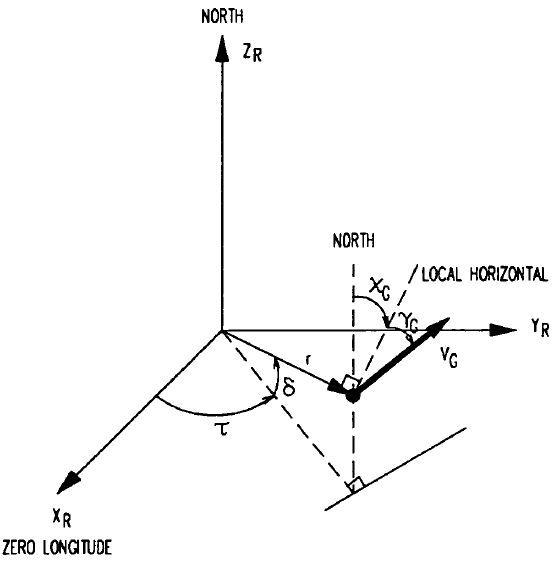
\includegraphics[width=0.4\textwidth]{figures/launcher_methods/spherical_mooij1994motion.jpg}
%\caption{Graphical definition of the spherical coordinate system. The angles are all defined positive in the direction of the arrow\cite{mooij1994motion}}
%\label{fig:spherical_mooij1994motion}
%\end{figure} 

\begin{figure}[!ht]
\centering
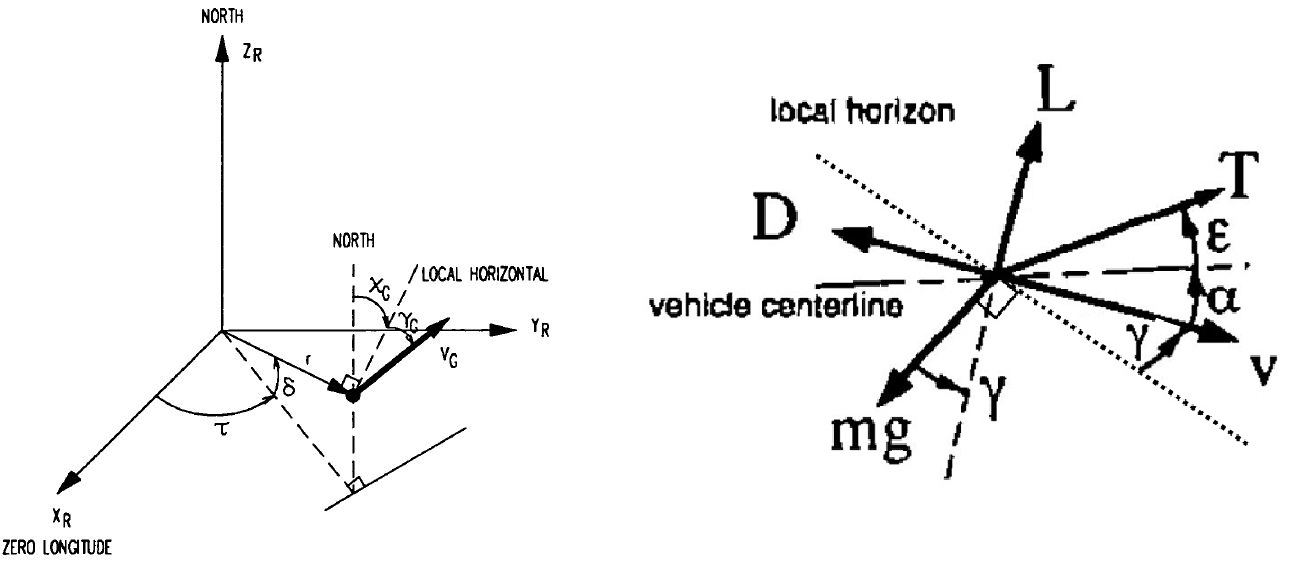
\includegraphics[width=0.7\textwidth]{figures/launcher_methods/spherical_mooij1994motion_force_model_fanning1996model.jpg}
\caption{(Left) Graphical definition of the 3D spherical coordinate system. The angles are all defined positive in the direction of the arrow\cite{mooij1994motion} (Right) 2D graphical definition of the force model \cite{fanning1996model}.}
\label{fig:spherical_mooij1994motion_force_model_fanning1996model}
\end{figure}

It was decided to use the Cartesian coordinate system for the simulation. The results of each iteration (position and velocity) can easily be transformed to spherical coordinates (see \Cref{ch:reftrans}) to gain more insight into the trajectory. When formulating the \ac{EoM} the definition of the different forces acting on the \ac{MAV} are required (the \ac{EoM} will then be formulated using the Cartesian coordinates). A two-dimensional representation of the forces acting on the \ac{MAV} is provided in \Cref{fig:spherical_mooij1994motion_force_model_fanning1996model} (Right). In this case it will be assumed that there is no wind acting on the \ac{MAV}. This can be done, because wind is random and can not be predicted easily. 
%
%because the atmosphere is very thin and because a simplified model will make it easier for the optimiser to converge, since convergence will be less and less likely if there are increasingly more optimisation parameters. 


%\begin{figure}[!ht]
%\centering
%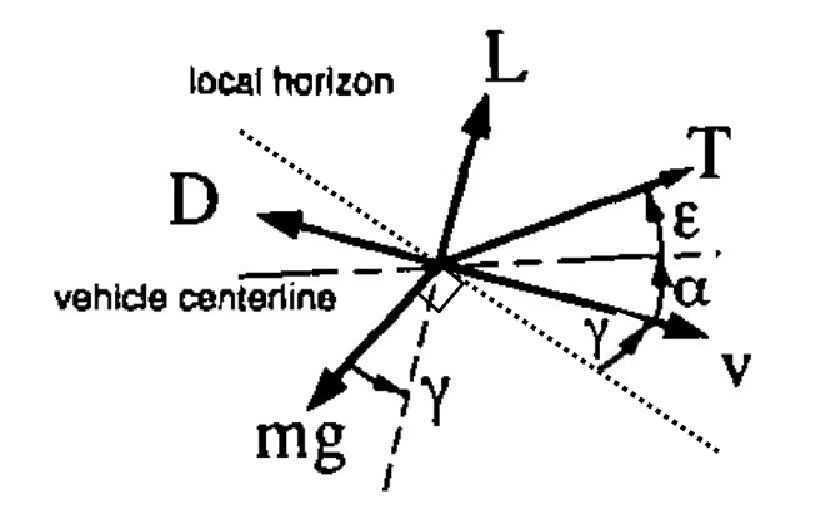
\includegraphics[width=0.4\textwidth]{figures/launcher_methods/force_model_fanning1996model.jpg}
%\caption{Graphical definition of the force model \cite{fanning1996model}}
%\label{fig:force_model_fanning1996model}
%\end{figure} 

\nomenclature[R5]{$L$}{Lift \nomunit{N}}
\nomenclature[R1]{$D$}{Drag \nomunit{N}}
\nomenclature[Ra2]{$T$}{Thrust \nomunit{N}}
\nomenclature[R5]{$m$}{Mass \nomunit{kg}}
\nomenclature[R3]{$g$}{Local gravitational acceleration \nomunit{m/s$^{2}$}}
\nomenclature[G3]{$\epsilon_{T}$}{Thrust elevation-gimbal angle  \nomunit{rad}}

In the model presented in \Cref{fig:spherical_mooij1994motion_force_model_fanning1996model} $\epsilon$ (from now on $\epsilon_{T}$) is the thrust elevation-gimbal angle and the lift $L$, drag $D$ and thrust $T$ are defined by \Cref{eq:l_d_t} \cite{wittenberg2014rocket}. 

To simulate out-of-plane motion and thus making it a three-dimensional model, a second thrust-gimbal angle is introduced as seen in \Cref{fig:propframe2_mooij1994motion}. This angle is defined in the x-y plane of the body frame, or B-frame, where it should be noted that the positive x-axis is defined through the vehicle centreline in the direction of flight, the z-axis is defined pointing down in \Cref{fig:spherical_mooij1994motion_force_model_fanning1996model} (left) perpendicular to the vehicle centreline and the y-axis is then pointing out of the x-z plane by the convention of the right-hand-rule \acsu{RHR}. This second gimbal angle is called the thrust azimuth gimbal angle $\psi_{T}$ as by \cite{mooij1994motion}.

\begin{figure}[!ht]
\centering
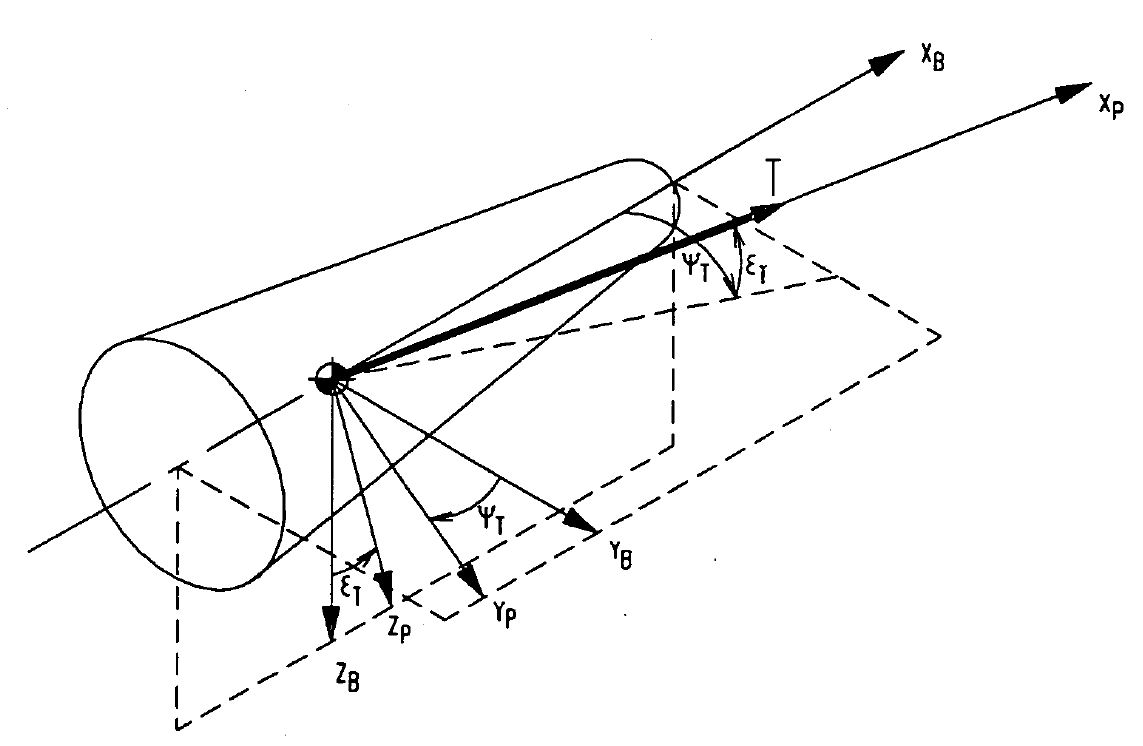
\includegraphics[width=0.6\textwidth]{figures/reference_frames/propframe_mooij1994motion.jpg}
\caption{Definition of the thrust angles \cite{mooij1994motion}.}
\label{fig:propframe2_mooij1994motion}
\end{figure}

\nomenclature[G9]{$\psi_{T}$}{Thrust elevation-gimbal angle  \nomunit{rad}}

In the equations for $L$, $D$ and $T$, $\rho$ is the atmospheric density, $S$ is the reference surface area, $C_{L}$ the lift coefficient, $C_{D}$ the drag coefficient, $\dot{m}$ the mass flow rate $\left(=-\dfrac{dm}{dt}\right)$, $g_{0}$ the gravitational acceleration at Earth sea-level (not Mars), $c_{eff}$ the effective expulsion velocity, $w_{e}$ the expulsion velocity, $A_{e}$ the exit surface area of the nozzle, $p_{e}$ the exit pressure and $p_{0,s}$ the pressure of the surrounding air. 


\begin{equation} \label{eq:l_d_t}
\begin{split}
L&=\dfrac{1}{2}\rho V^{2}S C_{L}\\
D&=\dfrac{1}{2}\rho V^{2}S C_{D}\\
T&=\dot{m}g_{0}I_{sp}=\dot{m}c_{eff}=\dot{m}w_{e}+A_{e}\left(p_{e}-p_{0,s}\right)\\
\end{split}
\end{equation}


\nomenclature[G6]{$\rho$}{Atmospheric density \nomunit{kg/m$^{3}$}}
\nomenclature[Ra1]{$S$}{Surface area \nomunit{m$^{2}$}}
\nomenclature[R1]{$C_{L}$}{Lift coefficient \nomunit{-}}
\nomenclature[R1]{$C_{D}$}{Drag coefficient \nomunit{-}}
\nomenclature[R6]{$\dot{m}$}{Mass flow rate \nomunit{kg/s}}
\nomenclature[C]{$g_{0}$}{Gravitational acceleration at Earth sea-level [9.81] \nomunit{m/s$^{2}$}}
\nomenclature[R]{$c_{eff}$}{Effective expulsion velocity \nomunit{m/s}}
\nomenclature[Ra3]{$w_{e}$}{Expulsion velocity \nomunit{m/s}}
\nomenclature[R]{$A_{e}$}{Exit surface area of the nozzle \nomunit{m$^{2}$}}
\nomenclature[R9]{$p_{e}$}{Exit pressure \nomunit{Pa}}
\nomenclature[R9]{$p_{0,s}$}{Pressure of the surrounding air \nomunit{Pa}}
\nomenclature[R4]{$h$}{Altitude \nomunit{m}}


All these equations depend on the altitude $h$: $\rho=f\left(h\right)$ and $p_{0,s}=f\left(h\right)$. Also, both coefficients are a function of the Mach number $M$ and the angle of attack $\alpha$. In this thesis problem, it is assumed that $\alpha=0^{\circ}$ (also see \Cref{subsec:coreom_mav}). This means that the drag coefficient is only a function of the Mach number. If a simple "pencil" shape is assumed, which is a reasonable assumption when examining the baseline model in \Cref{fig:baseline_mav_trinidad2012}, then \cite{whitehead2004mars} provides an estimation of the drag coefficient for different Mach numbers as can be seen in \Cref{fig:dragcoeff_whitehead2004mars}. 

\begin{figure}[!ht]
\centering
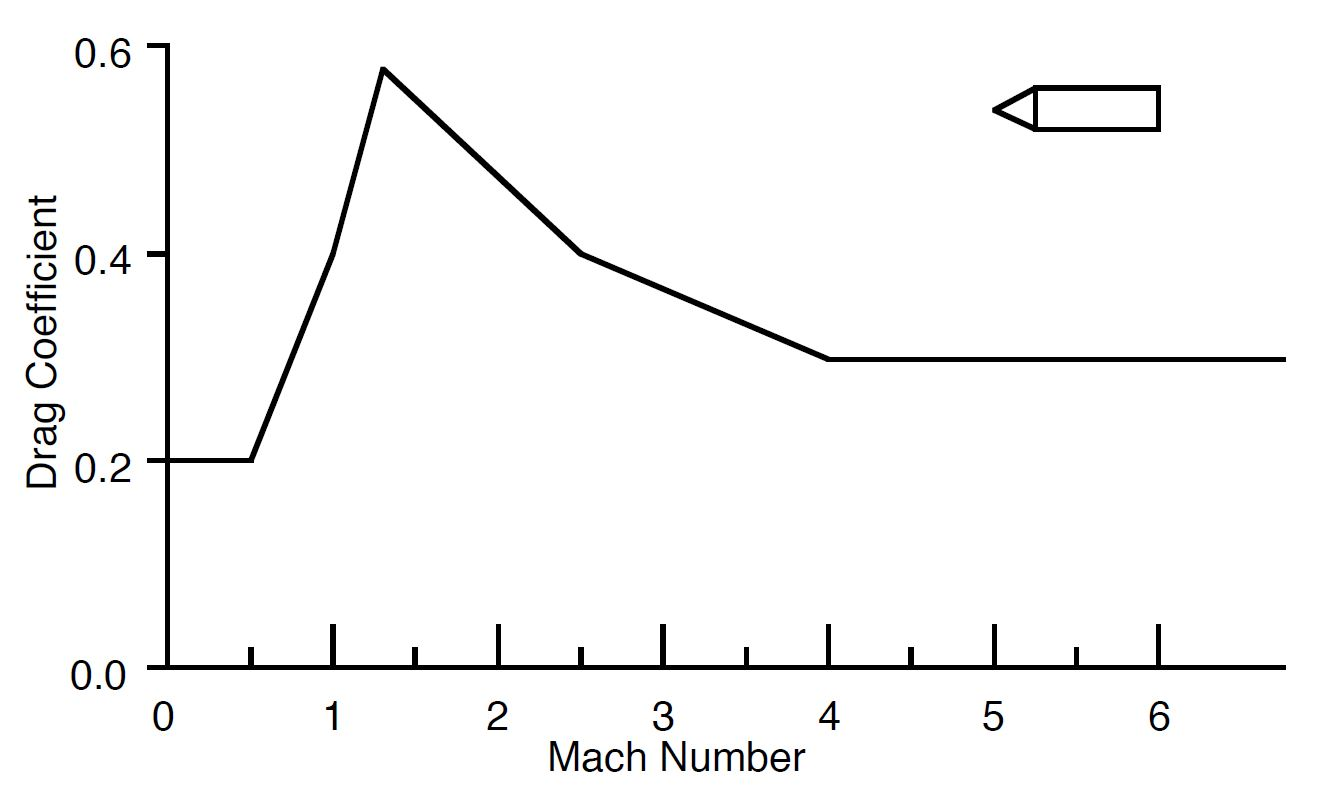
\includegraphics[width=0.4\textwidth]{figures/launcher_methods/dragcoeff_whitehead2004mars.jpg}
\caption{Drag coefficient as a function of Mach number \cite{whitehead2004mars}.}
\label{fig:dragcoeff_whitehead2004mars}
\end{figure} 

\nomenclature[R]{$a$}{Local speed of sound  \nomunit{m/s}}
\nomenclature[R8]{$M$}{Mach number \nomunit{-}}
\nomenclature[G]{$\alpha$}{Angle of attack \nomunit{rad}}

This drag coefficient plot can be used to determine the drag at different velocities (since $M=f\left(V,a\right)$ where $a$ is the speed of sound in the Martian atmosphere at that particular point which can be obtained through the atmospheric model that will be chosen). Thus given a certain atmospheric model, the air density and pressure at different altitudes and the Mach number can be computed. The atmospheric model will be selected and discussed in \Cref{ch:mars-atm-mod}. \\




The gravity force $mg$ depends on the local gravitational acceleration $g$. This $g$ can be determined assuming a homogeneous gravity field and a spherical Mars in the rotating Mars \ac{RF} using \Cref{eq:homo_square} where $g_{M0}$ is the standard gravitational acceleration on the surface of Mars (3.71 m/s$^{2}$)\footnote{All constants from NASA Mars fact sheet \cite{williams2015} unless otherwise mentioned} , $R_{M}$ is the (local) radius of Mars (3389.5 km), $G$ the gravitational constant (6.67408$\cdot$10$^{-11}$m$^{3}$/(kg$\cdot$s$^{2}$)), $M_{M}$ the mass of Mars (6.4174$\cdot$10$^{23}$ kg), $\mu_{M}$ the standard gravitational parameter of Mars (4.283$\cdot$10$^{13}$ m$^{3}$/s$^{2}$) and $r$ the position radius of the vehicle. The $J_{2}$ for Mars is equal to 1960.45$\cdot$ 10$^{-6}$ \cite{williams2015}, which would result in an average acceleration in the radial direction (same as gravity) in the order of 10$^{-2}$ m/$s^{2}$ (assuming an ascent time of 5 minutes and based on the equations provided in \cite{noomen2011kepler}). This in turn translates to a $\Delta V$ in the order of 10$^{0}$ m/s and a $\Delta r$ in the order of 10$^{3}$ m. This difference is so small that the perturbations due to irregularities in Mars' gravity field (J2, J3, etcetera) can be neglected.

\begin{equation} \label{eq:homo_square}
g=g_{M0}\left(\dfrac{R_{M}}{r}\right)^{2}=-\dfrac{GM_{M}}{r^{2}}=-\dfrac{\mu_{M}}{r^{2}}
\end{equation}

\nomenclature[C1]{$R_{M}$}{(Local) radius of Mars [3389500] \nomunit{m}}




%can however be determined (or rather modelled) in different ways. On the surface of the planet, either the standard gravitational acceleration for Mars $g_{M0}$ can be taken for the entire planet or a more accurate gravity model can be taken to simulate the proper launch site conditions (depending on the position). An example of such a model based on data gathered by the \ac{MRO} is the MSM2011 model presented by \cite{hirt2012kilometer}. The maximum and minimum gravitational accelerations are 3.743 and 3.683 m/s$^{2}$ respectively, which is only a difference of 0.06 m/s$^{2}$. In comparison, $g_{M0}$ reported by NASA \cite{williams2015}, has a value of 3.71 m/s$^{2}$, which is approximately the average of the afore mentioned values. If $g_{M0}$ is chosen for the entire (spherical) planet then \Cref{eq:homo_square} can be used to compute the gravitational acceleration at a given altitude for a homogeneous gravity field \cite{fanning1996model} where $R_{M}$ is the (local) radius of Mars. The same equation can be used with the more detailed gravitational model (then $g_{M0}$ is replaced by $g_{local,surface}$), but then the local gravity depends on the position of the \ac{MAV} on or above the planet while still using the square gravity law. 
%
%\begin{equation} \label{eq:homo_square}
%g=g_{M0}\left(\dfrac{R_{M}}{r}\right)
%\end{equation}

%\nomenclature{$R_{M}$}{(Local) radius of Mars \nomunit{m}}
%
%\Cref{eq:homo_square} can also be written in its original form such that the local gravity at any point on or above Mars can be computed, using a homogeneous gravity field, as a function of the gravitational constant $G$ and the mass of Mars $M_{M}$ as is shown in \Cref{eq:homo_square_gm}. $GM_{M}$ can also be written as $\mu_{M}$ which is the standard gravitational parameter of Mars.

\nomenclature[C1]{$M_{M}$}{Mass of Mars [6.4174$\cdot$10$^{23}$] \nomunit{kg}} %[6.4174$\cdot$10$^{23}$] \cite{williams2015}
\nomenclature[C1]{$G$}{Gravitational constant [6.6744585$\cdot$10$^{-11}$]   \nomunit{m$^{3}$/(kg$\cdot$s$^{2}$)}} %[6.6744585$\cdot$10$^{-11}$] \cite{williams2015}
%\nomenclature{$\mu_{M}$}{Standard gravitational parameter of Mars  \nomunit{m$^{3}$/s$^{2}$}}


%\begin{equation} \label{eq:homo_square_gm}
%g=\dfrac{GM_{M}}{r^{2}}
%\end{equation}

This equation can then be used to determine the gravitational acceleration at any distance from Mars. It is assumed that the mass of the \ac{MAV}, the orbiter(s) and the two Martian moons can be neglected with respect to the mass of Mars (the mass of Phobos is an order of 7 smaller than the mass of Mars) \cite{williams2015} so third-body perturbations are not considered. Also, during the ascent the perturbations due to irregularities in Mars' gravity field can be neglected, because the time spent in ascent is relatively short.

% This simplified model for the gravity is preferred over the inclusion of gravitational perturbations (resulting in the more accurate model for the local gravity) because the effect of these gravitational perturbations $J$ are small during an ascent. 

\subsection{Corresponding \ac{EoM} and initial assumptions}
\label{subsec:coreom_mav}
The general equations of motion can be derived using the described model, and are based on \cite{mooij1994motion}. Because the motion of the Mars 2022 orbiter will be described in an inertial Mars frame and because the final orbit will be described using Kepler elements it is useful to write the \ac{EoM} for the \ac{MAV} ascent in the same frame. The current conditions can be described as shown by \Cref{eq:current_conditions}, where $m_{MAV}$ is the mass of the \ac{MAV} and the subscript $I$ refers to the inertial frame.

\begin{align} \label{eq:current_conditions}
\mathbf{r}&=\begin{pmatrix}
x_{I}\\
y_{I}\\
z_{I}\\
\end{pmatrix}
&
\mathbf{V}&=\begin{pmatrix}
V_{x_{I}} \\
V_{y_{I}} \\
V_{z_{I}}\\
\end{pmatrix}
&
m_{MAV}&
\end{align}

\nomenclature[R7]{$m_{MAV}$}{\ac{MAV} mass \nomunit{kg}}

The \ac{EoM} can now be described by \Cref{eq:cart_eom_mav}. Here, $a$ represents the acceleration.

\begin{align} \label{eq:cart_eom_mav}
\begin{split} 
\dot{x}_{I}&=V_{x_{I}}\\
\dot{y}_{I}&=V_{y_{I}}\\
\dot{z}_{I}&=V_{z_{I}}
\end{split} 
&
\begin{split}
\ddot{x}_{I}&=\dot{V}_{x_{I}}=a_{x_{I}}\\
\ddot{y}_{I}&=\dot{V}_{y_{I}}=a_{y_{I}}\\
\ddot{z}_{I}&=\dot{V}_{z_{I}}=a_{z_{I}}
\end{split}
&
\dot{m}_{MAV}=-\dfrac{T}{g_{0}I_{sp}}
\end{align}

\nomenclature[R]{$a$}{Acceleration \nomunit{m/s$^{2}$}}

% and accelerations 

The accelerations follow from Newton's $F=m \cdot a$ and can thus be described as a function of the mass and the different forces acting on the \ac{MAV}. These are all described in different reference frames unfortunately, which means that the forces acting on the \ac{MAV} will have to be translated into the inertial Mars frame. This is done through reference frame transformations (which was discussed in detail in \Cref{ch:reftrans}). A transformation is always performed by rotating around the different axes in a particular order which requires the different rotational angles. Each rotation around a certain axis has a corresponding transformation matrix, for instance $\mathbb{T}_{\mathbf{x}}(\phi)$ where $\mathbb{T}$ is the symbol for a transformation matrix, the subscript $x$ shows that it is a rotation around the x-axis and the $\phi$ is in this case the angle of rotation. This particular rotation is a positive rotation around the x-axis (following the \ac{RHR}). Should the rotation be negative then the transformation matrix would have been presented as $\mathbb{T}_{\mathbf{x}}(-\phi)$. First it is important to define the reference frames in which the different forces are acting. In this case the thrust is acting in a propulsion frame or P-frame (with the corresponding gimbal angles as rotation angles), the drag is acting in the aerodynamic frame or A-frame and the gravity is acting in the Mars rotational frame or R-frame. Before describing the relation between the different frames, a number of assumptions are made.

\begin{itemize}
\item No wind; it is assumed that there is no wind and thus no corresponding effects or changes in the \ac{MAV} attitude to simplify the simulation. This also means that during the verification of the program, wind will not be taken into account.
\item No angle of attack; the angle of attack is assumed to be zero, the \ac{MAV} is assumed to always move in the direction of flight. 
\item No lift; it can be assumed that there is no lift, based on the assumption that there is no angle of attack and that the \ac{MAV} has a symmetric shape.
\item No bank angle; because the system is a point mass system and since there is no lift, the bank angle can be assumed equal to zero \cite{kesteren2013air}.
\item No side-slip; because there is no wind and no banking, there will be no side-slip. Therefore the side-slip angle can be assumed to be zero \cite{mooij1994motion}.
%\item $\epsilon$ = 0; Since the baseline engines can not be gimballed, the gimbal angle can be set equal to zero \cite{trinidad2012}


\end{itemize}

%\nomenclature{$\gamma$}{Flight-path angle \nomunit{rad}}
%\nomenclature{$\chi$}{Azimuth (or heading angle) \nomunit{rad}}

From these assumptions it is clear that the A-frame is in this case identical to the body frame or B-frame. Therefore the body is always pointing into the same direction as the velocity vector. This provides another set of angles to transform to the inertial frame as can be seen in \Cref{fig:spherical_mooij1994motion_force_model_fanning1996model}. These angles are the flight-path angle and the heading angle. The subscript $G$ shows that this frame is set-up for the flight-path angle, azimuth and velocity based on the ground-speed as opposed to airspeed, but since there is no wind this is irrelevant in this case. Rotating over these angles would result in transforming to the vertical frame or V-frame. In the vertical frame the x-axis points towards the northern hemisphere, the z-axis points towards the centre of mass of the orbiting body and the y-axis points towards the east \cite{mooij1994motion}. \Cref{fig:spherical_mooij1994motion_force_model_fanning1996model} then also shows the rotation angles required to transform from the V-frame to the R-frame. These angles are the latitude $\delta$ and the longitude $\tau$ in a rotating frame. The final transformation involves the rotation from the R-frame to the I-frame. This rotation depends on the location of the prime meridian (the meridian of zero longitude) at the time that the inertial reference frame was set $\Omega_{P}$, the rotational velocity of Mars $\dot{\Omega}_{M}$ and the time between when the inertial frame was set and the current time $t_{O}$. The rotational angle between the R-frame and the I-frame can then be defined to be $\dot{\Omega}_{M}t_{O}-\Omega_{P}$ (where the motion and angles are defined towards the east). 
Now including all the forces, accelerations and rotations and using the notation for transformation matrices as defined earlier, the expressions for the accelerations in the I-frame can be described by \Cref{eq:acc_ascent}. In this notation, each vertical line depicts when a new reference frame is reached and the letter shows which one. Also, because the transformations require matrix multiplications, the transformation should be executed from right to left.

\nomenclature[C]{$\dot{\Omega}_{M}$}{Rotational velocity of Mars [7.088$\cdot$10$^{-5}$] \nomunit{rad/s}}
\nomenclature[Ra1]{$t_{O}$}{Time from inertial reference frame definition \nomunit{s}}
\nomenclature[Ga1]{$\Omega_{P}$}{Prime meridian offset at inertial reference frame definition  \nomunit{rad}}



\begin{multline} \label{eq:acc_ascent}
\begin{pmatrix}
a_{x_{I}}\\
a_{y_{I}}\\
a_{z_{I}}\\
\end{pmatrix}
=
\Bigg|_{\mathbf{I}}\mathbb{T}_{\mathbf{z}}\left(-\dot{\Omega}_{M}t_{O}+\Omega_{P}\right)\Bigg|_{\mathbf{R}}\left[
\begin{pmatrix}
-\mu_{M}\dfrac{x_{R}}{r^{3}}\\
-\mu_{M}\dfrac{y_{R}}{r^{3}}\\
-\mu_{M}\dfrac{z_{R}}{r^{3}}\\
\end{pmatrix}
+\Bigg|_{\mathbf{R}}\mathbb{T}_{\mathbf{z}}\left(-\tau\right)\mathbb{T}_{\mathbf{y}}\left(\dfrac{\pi}{2}+\delta\right)\Bigg|_{\mathbf{V}}\mathbb{T}_{\mathbf{z}}\left(-\chi\right)\mathbb{T}_{\mathbf{y}}\left(-\gamma\right)\Bigg|_{\mathbf{B}}\left\lbrace
\begin{pmatrix}
-\dfrac{D}{m_{MAV}}\\
0\\
0\\
\end{pmatrix}
+ \right. \right. \dots \\
\dots +
\left. \left.
\Bigg|_{\mathbf{B}}\mathbb{T}_{\mathbf{z}}\left(-\psi_{T}\right)\mathbb{T}_{\mathbf{y}}\left(-\epsilon_{T}\right)\Bigg|_{\mathbf{P}}
\begin{pmatrix}
\dfrac{T}{m_{MAV}}\\
0\\
0\\
\end{pmatrix}
\right\rbrace
\right]
\end{multline}

The corresponding transformation matrices were already written out in \Cref{ch:reftrans}. Also, the position and velocity will change each time step, which means that the angles $\tau$, $\delta$, $\chi$ and $\gamma$ will also change. These angles can all be described in the R-frame. Thus to determine the updated values, the position and velocity will have to be transformed from the I-frame to the R-frame. Then using the transformation between Cartesian and spherical coordinates, the angles can be obtained. This transformation was also described in \Cref{ch:reftrans}. Following from the haversine formula based on great circles, the change in the ground distance travelled $S_{G}$ (in the R-frame) can be computed as a function of the longitude and latitude as shown by \Cref{eq:ground_dist}. 

\begin{equation} \label{eq:ground_dist}
\dot{S}_{G}=2R_{M}\arcsin\left(\sqrt{\sin^{2}\left(\dfrac{\dot{\delta}}{2}\right)+\frac{1}{2}\left(\cos\left(\dot{\delta}\right)+\cos\left(2\delta+\dot{\delta}\right)\right)\sin^{2}\left(\dfrac{\dot{\tau}}{2}\right)}\right)
\end{equation}

\nomenclature[Ra1]{$S_{G}$}{Travelled ground distance  \nomunit{m}}


\section{Required launch trajectory}
\label{sec:reqlaunchtraj}
When examining the different possible launch trajectories, one mainly looks at different ways to control the ascent vehicle in such a manner that reduces losses. Four different possible launch trajectories (usually followed by each other) are a vertical rise phase, a constant pitch-rate phase, a constant pitch phase and a gravity-turn phase. Also, sometimes a control program for the pitch/pitch-rate is followed instead of a constant pitch/pitch-rate. The pitch angle is defined as $\alpha+\gamma$, however since there is no angle of attack in this case, the pitch angle is equal to the flight-path angle $\gamma$ (in the R-frame and V-frame). The ascent is then followed by a coasting phase and a final burn phase to place the \ac{s/c} into a desired orbit \cite{di2007system,fanning1996model,wittenberg2014rocket,pagano2010thesis}. In this case however, since it is assumed that the engines can be gimballed ($\psi_{T}$ and $\epsilon_{T}$) the phase between the vertical rise and the gravity-turn can be optimised and does not need a constant pitch-rate and constant pitch phase. This transition phase shall be known as the first thruster control phase. When all the propellants of the first stage are used, the stage-separation will take place (which often happens during the gravity-turn (see \Cref{subsec:asc_grav_turn})). Then the second stage ignites and will continue the gravity-turn. At some point in the second stage burn, it could be more beneficial to change the flight program to a second thruster control phase. This is to avoid an early zero flight-path angle and to position the \ac{MAV} such that a certain apocentre can be reached. After the second stage is burned out, the coasting phase will start. At the end of this coasting phase (at apocentre of the ascent) a final burn is provided to propel the \ac{MAV} into the desired final orbit. It should, however, be noted that a vertical rise might not be optimal, which is why the set of equations mentioned in \Cref{eq:acc_ascent} allow for an initial heading ($\chi$) and launch angle ($\gamma$) to be defined at the beginning of the simulation. The different ascent phases will be discussed in this section.

\subsection{Vertical rise}
\label{subsec:asc_ver_rise}
The vertical rise phase can be used to penetrate the thickest layers of the atmosphere before performing the gravity-turn \cite{fanning1996model,wittenberg2014rocket}. This will reduce the effect of drag significantly but will increase the gravity losses.  During the vertical ascent the flight-path angle is equal to 90$^{\circ}$ (or $\dfrac{\pi}{2}$). The heading angle during this phase is undefined, which means that the orientation of the \ac{MAV} is not defined at this stage. Also, during the vertical ascent both gimbal angles are set equal to zero. Therefore the flight-path angle and heading angle do not change during the vertical ascent and since the value of the heading angle is not important, it can be set equal to zero. As soon as the first thruster control phase starts, the heading angle will be defined automatically as a result of the gimbal angles, and the flight-path angle will change as well. With these trajectory characteristics the expressions in \Cref{eq:acc_ascent} can be rewritten for the vertical phase (see \Cref{eq:vert_eom_ascent}). It is worth mentioning that the first two rotations are now both around the y-axis, which means that they can be performed at once (resulting in a positive rotation $\delta$) however, for clarity it is written such that the V-frame is included.


\begin{equation} \label{eq:vert_eom_ascent}
\begin{pmatrix}
a_{x_{I}}\\
a_{y_{I}}\\
a_{z_{I}}\\
\end{pmatrix}
=
\Bigg|_{\mathbf{I}}\mathbb{T}_{\mathbf{z}}\left(-\dot{\Omega}_{M}t_{O}+\Omega_{P}\right)\Bigg|_{\mathbf{R}}\left[
\begin{pmatrix}
-\mu_{M}\dfrac{x_{R}}{r^{3}}\\
-\mu_{M}\dfrac{y_{R}}{r^{3}}\\
-\mu_{M}\dfrac{z_{R}}{r^{3}}\\
\end{pmatrix}
+\Bigg|_{\mathbf{R}}\mathbb{T}_{\mathbf{z}}\left(-\tau\right)\mathbb{T}_{\mathbf{y}}\left(\dfrac{\pi}{2}+\delta\right)\Bigg|_{\mathbf{V}}\mathbb{T}_{\mathbf{y}}\left(-\dfrac{\pi}{2}\right)\Bigg|_{\mathbf{B}}
\begin{pmatrix}
\dfrac{T-D}{m_{MAV}}\\
0\\
0\\
\end{pmatrix}
\right]
\end{equation}

For the optimisation of this phase the only control variable can be the vertical ascent time $t_{v}$ (if not pre-set). 

\subsection{First thruster control phase}
\label{subsec:first_thrust_cont}
To transition from the vertical phase to the gravity-turn, a change in the heading and flight-path angle is required. These changes can be set in motion by gimballing the thruster, or in other words by providing a thrust elevation ($\epsilon_{T1}$, where the subscript 1 refers to the first thruster control phase) and/or thrust azimuth angle ($\psi_{T1}$). These two angles are both optimisation parameters. In this case, it is necessary to use the complete set of equations for the accelerations (\Cref{eq:acc_ascent}). A third optimisation parameter for the first thruster control phase is the time spent in this phase $t_{T1}$. During this phase a reduced thrust could be required. This would then introduce another optimisation parameter: the thrust level during the first thruster control phase $T_{T1}$. At the end of this phase, the thrust level is again set to full thrust (if it was changed) and both $\epsilon_{T1}$ and $\psi_{T1}$ are again set to zero which will be the start of the gravity-turn phase.\\
The current baseline design does not assume an engine that can be gimballed (see \Cref{sec:mav_des}), but uses control thrusters instead. However, for this thesis it can be assumed that in the future either gimballing will be introduced on the \ac{MAV} or the trajectory adjustments will indeed have to be made by control thrusters instead.




\subsection{Gravity-turn and second thruster control phase}
\label{subsec:asc_grav_turn}
After the vertical rise and the first thruster control phase, a so-called gravity-turn is initiated. The gravity-turn results in a rotation of the \ac{MAV} into a (near) horizontal flight orientation which reduces the gravity losses and is usually initiated after passing through the thickest layers of the atmosphere to reduce drag. Because at the beginning of this phase the flight-path angle is $0\leq \gamma\leq \dfrac{\pi}{2}$ (in the R-frame), the gravity force will cause a change in this flight-path angle. This will cause the \ac{MAV} to turn towards a lower flight-path angle automatically without the use of the gimbal feature. Therefore, during this manoeuvre, the gimbal angles are both zero, which means that the thrust is again acting directly in the B-frame simplifying the acceleration equation. However, in this case there is a flight-path angle and there is also a heading angle. The resulting acceleration equation can be represented by \Cref{eq:grav_acc_eom}.

\begin{equation} \label{eq:grav_acc_eom}
\begin{pmatrix}
a_{x_{I}}\\
a_{y_{I}}\\
a_{z_{I}}\\
\end{pmatrix}
=
\Bigg|_{\mathbf{I}}\mathbb{T}_{\mathbf{z}}\left(-\dot{\Omega}_{M}t_{O}+\Omega_{P}\right)\Bigg|_{\mathbf{R}}\left[
\begin{pmatrix}
-\mu_{M}\dfrac{x_{R}}{r^{3}}\\
-\mu_{M}\dfrac{y_{R}}{r^{3}}\\
-\mu_{M}\dfrac{z_{R}}{r^{3}}\\
\end{pmatrix}
+\Bigg|_{\mathbf{R}}\mathbb{T}_{\mathbf{z}}\left(-\tau\right)\mathbb{T}_{\mathbf{y}}\left(\dfrac{\pi}{2}+\delta\right)\Bigg|_{\mathbf{V}}\mathbb{T}_{\mathbf{z}}\left(-\chi\right)\mathbb{T}_{\mathbf{y}}\left(-\gamma\right)\Bigg|_{\mathbf{B}}
\begin{pmatrix}
\dfrac{T-D}{m_{MAV}}\\
0\\
0\\
\end{pmatrix}
\right]
\end{equation}

At the start of the gravity-turn, there is also a certain heading angle. This heading angle (in the I-frame) will determine the final inclination of the orbit together with the \ac{MAV} latitude at the start of the gravity-turn. The relation for the inclination is shown by \Cref{eq:heading_incl_rel}. During the gravity-turn (and the rest of the ascent phase) both the heading angle and latitude will change, however the eventual inclination which the \ac{MAV} will reach will stay the same (assuming $\psi_{T2}$ = 0 during the second thruster control phase). If at the beginning of the gravity-turn, the desired inclination has not been reached, it means that the first two phases were not ideal and will have to be changed. Also, in this case the inclination is an optimisation parameter since different orbital inclinations will have to be investigated combined with the Mars 2022 orbiter trajectory.


\begin{equation} \label{eq:heading_incl_rel}
\chi_{0}=\arcsin\left(\dfrac{\cos\left(i\right)}{\cos\left(\delta_{0}\right)}\right)
\end{equation}

\nomenclature[R4]{$i$}{Inclination  \nomunit{rad}}



At some point the first stage will burn out (which often happens during the gravity-turn), be ejected (simulated by an instant reduction in mass; the empty mass of stage 1) and the second stage will be ignited and burn until its burn-out. Should this separation happen during the gravity-turn, the second stage could either continue following this trajectory, follow a second thruster control program or both. Because there is no need to change the inclination (which was already set by the first thruster control phase) this second thruster control phase will only use the elevation-gimbal angle $\epsilon_{T2}$ to change the \ac{MAV} attitude, resulting in the acceleration equation given by \Cref{eq:second_thrust_eom}.

\begin{multline} \label{eq:second_thrust_eom}
\begin{pmatrix}
a_{x_{I}}\\
a_{y_{I}}\\
a_{z_{I}}\\
\end{pmatrix}
=
\Bigg|_{\mathbf{I}}\mathbb{T}_{\mathbf{z}}\left(-\dot{\Omega}_{M}t_{O}+\Omega_{P}\right)\Bigg|_{\mathbf{R}}\left[
\begin{pmatrix}
-\mu_{M}\dfrac{x_{R}}{r^{3}}\\
-\mu_{M}\dfrac{y_{R}}{r^{3}}\\
-\mu_{M}\dfrac{z_{R}}{r^{3}}\\
\end{pmatrix}
+\Bigg|_{\mathbf{R}}\mathbb{T}_{\mathbf{z}}\left(-\tau\right)\mathbb{T}_{\mathbf{y}}\left(\dfrac{\pi}{2}+\delta\right)\Bigg|_{\mathbf{V}}\mathbb{T}_{\mathbf{z}}\left(-\chi\right)\mathbb{T}_{\mathbf{y}}\left(-\gamma\right)\Bigg|_{\mathbf{B}}\left\lbrace
\begin{pmatrix}
-\dfrac{D}{m_{MAV}}\\
0\\
0\\
\end{pmatrix}
+ \right. \right. \dots \\
\dots +
\left. \left.
\Bigg|_{\mathbf{B}}\mathbb{T}_{\mathbf{y}}\left(-\epsilon_{T}\right)\Bigg|_{\mathbf{P}}
\begin{pmatrix}
\dfrac{T}{m_{MAV}}\\
0\\
0\\
\end{pmatrix}
\right\rbrace
\right]
\end{multline}


This manoeuvre could also be chosen to begin some time after the ignition of the second stage. Another aspect that could be used for the optimisation is the coasting time between the separation of the first stage and the second stage. All these different options result in a number of optimisation parameters which can be chosen to be active or not (either optimised or set as a constant parameter). These parameters are: burn-time of the first stage $t_{1}$, the first coasting time between the first and second stage $t_{c1}$, the elevation-gimbal angle $\epsilon_{T2}$ (with possible thrust control $T_{T2}$), the burn-time of the second stage $t_{2}$ and (if chosen to delay the second thruster manoeuvre) the time at which the second thruster control step starts $t_{T2}$. 


\nomenclature[Ra1]{$t_{1}$}{First stage burn-time  \nomunit{s}}
\nomenclature[Ra1]{$t_{c1}$}{Initial-second stage coast time  \nomunit{s}}
\nomenclature[Ra1]{$t_{2}$}{Second stage burn-time  \nomunit{s}}
\nomenclature[Ra1]{$t_{T2}$}{Second thruster control phase start time  \nomunit{s}}



\subsection{Coasting and orbit burn}
\label{subsec:asc_coast_burn}
The final coasting phase starts at the second stage burn-out. There will still be some remaining propellant mass in the second stage at that point which will be used to perform the final orbit injection burn. The required propellant mass is a direct result of the necessary change in velocity required to propel the \ac{MAV} into its final orbit from the current coasting trajectory. To compute this propellant mass, first the apocentre and pericentre of the current (elliptic) trajectory have to be determined \cite{fanning1996model} (see \Cref{eq:apsis_asc}).

\begin{equation} \label{eq:apsis_asc}
r_{ap}=\dfrac{-\mu_{M}r\pm\sqrt{\left(\mu_{M}r\right)^{2}+r\left(rV^{2}-2\mu_{M}\right)\left(rV\cos\left(\gamma\right)\right)^{2}}}{rV^{2}-2\mu_{M}}
\end{equation}  

Here $r_{ap}$ represents the pericentre $r_{p}$ for the negative and apocentre $r_{a}$ for the positive sign. At this point, a check is performed to assure that the reached $r_{a}$ is equal to the radius of the desired orbit (in case of a circular target orbit) or equal to the pericentre of the desired orbit (in case of an elliptic target orbit). The general equations that can be used for this check are provided in \Cref{eq:peri_apo} \cite{wakker2010astro1} where $a$ and $e$ are the semi-major axis and eccentricity of the desired target orbit respectively, which can be optimisation parameters as well, and the underscore $c$ stands for check.

\nomenclature[Ra0]{$r_{p}$}{Pericentre  \nomunit{m}}
\nomenclature[Ra0]{$r_{a}$}{Apocentre  \nomunit{m}}
\nomenclature[R1]{$e$}{Eccentricity  \nomunit{-}}
\nomenclature[R]{$a$}{Semi-major axis  \nomunit{m}}

\begin{equation} \label{eq:peri_apo}
\begin{split}
r_{a,c}&=a\left(1+e\right)\\
r_{p,c}&=a\left(1-e\right)\\
\end{split}
\end{equation}

The velocity at the apocentre can then be computed using \Cref{eq:vel_apo}.

\begin{equation} \label{eq:vel_apo}
V_{a}=\sqrt{V^{2}-2\mu_{M}\left(\dfrac{1}{r}-\dfrac{1}{r_{a}}\right)}
\end{equation}

The required $\Delta V$ to reach the desired orbit is then given by \Cref{eq:req_ini_orb}.

\begin{equation} \label{eq:req_ini_orb}
\Delta V = V_{a}-\sqrt{\mu_{M}\left(\dfrac{2}{r_{a}}-\dfrac{1}{a_{target}}\right)}
\end{equation}

Now that the required velocity change is known, the corresponding required propellant mass $\Delta m_{b}$ can be computed through the use of Tsiolkovsy's equation as the difference between the mass of the second stage at burn-out $m_{2}$ and the final mass of the second stage $m_{2,f}$ after the orbit burn. The expression for $\Delta m_{b}$ is then provided by \Cref{eq:req_propm_burn}.

\nomenclature[G3]{$\Delta m_{b}$}{Required propellant mass for orbit insertion  \nomunit{kg}}
\nomenclature[R6]{$m_{2}$}{Second stage mass after burn-out  \nomunit{kg}}
\nomenclature[R7]{$m_{2,f}$}{Final second stage mass  \nomunit{kg}}

\begin{equation} \label{eq:req_propm_burn}
\Delta m_{b}=m_{2}\left(1-exp\left(\dfrac{-\Delta V}{g_{0}I_{sp}}\right)\right)
\end{equation}

During the coasting and the final burn, the only optimisation parameters are the eccentricity and the semi-major axis of the desired orbit. Thus the maximum number of optimisation parameters for the ascent phase is 14 and are: $t_{v}$, $t_{T1}$, $T_{T1}$, $\epsilon_{T1}$, $\psi_{T1}$, $t_{1}$, $t_{c1}$, $t_{2}$, $t_{T2}$, $\epsilon_{T2}$, $T_{T2}$, $a$, $e$ and $i$. Most of these parameters are free, but it can be chosen to fix some of these as well. The number of optimisation parameters can also be increased using the design space for the \ac{MAV} provided in \Cref{subsec:cur_des_rest} which would include the  dimensions of the \ac{MAV}. Also, to add more flexibility, more intermediate thrust angles could be set as optimisation parameters. This would simply add (or even mix up) the different kinds of trajectories.



\section{Mars 2020 landing site conditions}
\label{sec:2020_land_con}
In the beginning of August 2015 the second Workshop on the Mars 2020 Landing Site was held in Monrovia, California \footnote{\label{foot:landsite} Landing site workshop: \url{http://marsnext.jpl.nasa.gov/} [Accessed 19 November 2015]}. Directly following this workshop, a meeting was held to select eight potential landing sites for the Mars 2020 rover. These sites are (alphabetically) presented in \Cref{tab:potential_land_site_char} including the position data. Please note that the latitude and longitudes are within an accuracy of approximately 5 km.


\begin{table}[!ht]
\begin{center}
\caption{Current candidate landing sites (source:\ac{JPL})}
\label{tab:potential_land_site_char}
\begin{tabular}{|l|l|l|l|}
\hline 
\textbf{Landing site} 	& \textbf{Altitude w.r.t. MOLA geoid [km]} & \textbf{Latitude [$^\circ$N]} & \textbf{Longitude [$^\circ$E]} \\ \hline \hline
Columbia Hills/Gusev &-1.9 & -14.4 & 175.6\\ \hline
Eberswalde & -1.4 & -23.0 & 327.0 \\ \hline
Holden & -2.1 & -26.4 & 325.1 \\ \hline
Jezero & -2.5 & 18.5 & 77.4 \\ \hline
Mawrth & -2.3 & 24.0 & 341.1 \\ \hline
NE Syrtis & -2.2 & 17.8 & 77.1 \\ \hline
Nili Fossae & -0.6 & 21.0 & 74.5 \\ \hline
SW Melas & -1.9 & -12.2 & 290.0 \\ \hline
 
\end{tabular}
\end{center}
\end{table}

There are also several landing site constraints that are important to the thesis problem:

\begin{itemize}
\item \textbf{Elevation}  The elevation of the landing site must be below +0.5 km MOLA elevation, which is with respect to the MOLA geoid (defined to be at a radius of 3396 km \cite{smith1998relationship,smith2001mars,barlow2008mars}, not to be confused with the volumetric mean radius mentioned in \cite{williams2015}). %3396.2 km $\pm$160 m
\item \textbf{Latitude} The landing site latitude has to be between $\pm30^{\circ}$ of the equator.
%\item \textbf{Landing Ellipse} The current best landing ellipse would be 18 km long and 14 km wide. 
\end{itemize}

These constraints result in a band where the landing sites can be chosen. The location of the eight chosen potential landing sites are indeed located in this band as shown by \Cref{fig:mars2020_land_grant2015landing} $^{\ref{foot:landsite}}$.


%\begin{figure}[!ht]
%\centering
%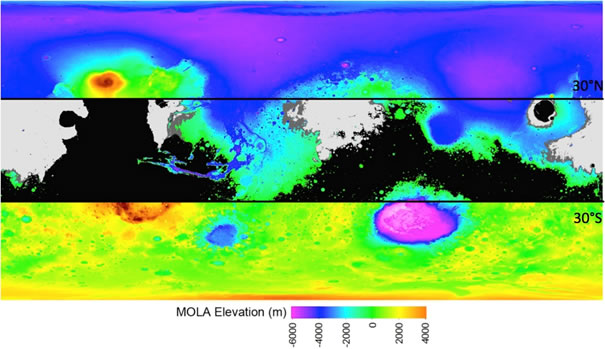
\includegraphics[width=0.6\textwidth]{figures/launcher_methods/constrained_area_grant2015landing.jpg}
%\caption{Constrained landing area on Mars between $30^{\circ}$N and $30^{\circ}$S. In that area, black land has an elevation above +0.5 km w.r.t. the MOLA geoid and the grey areas are lower thermal inertial constrained areas.}
%\label{fig:constrained_area_grant2015landing}
%\end{figure} 

\begin{figure}[!ht]
\centering
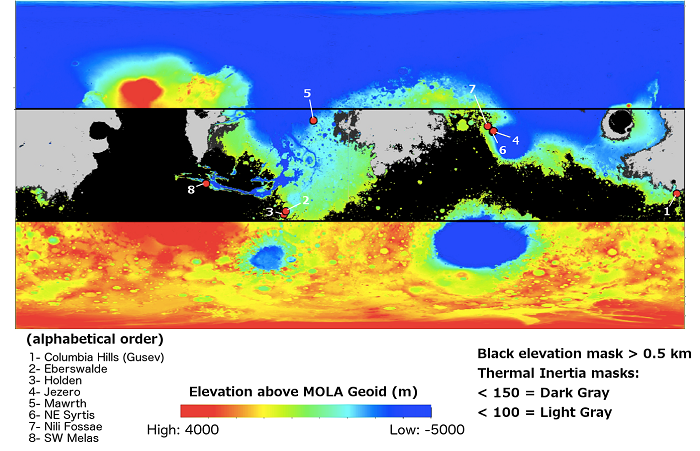
\includegraphics[width=1.0\textwidth]{figures/launcher_methods/mars2020_land_grant2015landing.png}
\caption{Locations of the eight potential landing sites within the constrained area.}
\label{fig:mars2020_land_grant2015landing}
\end{figure} 

The position data is all provided in the R-frame. With the different latitudes, the respective local rotational velocity $V_{y_{R,0}}$(due East or in the y-direction in the R-frame), as viewed from the I-frame can be determined. These velocities provide the values for the initial velocity vector. The relation for $V_{y_{R,0}}$ is given in \Cref{eq:init_east_vel_mav} and the initial velocity vector is then provided through \Cref{eq:init_vel_I_mav}. Here, $\dot{\Omega}_{M}$ is the rotational velocity of Mars, the L-frame is attached to the landing site and $R_{M}$ is the (local) radius of Mars.

\begin{equation} \label{eq:init_east_vel_mav}
V_{y_{R,0}}=\dot{\Omega}_{M}R_{M}\cos\left(\delta_{0}\right)
\end{equation}

\begin{equation} \label{eq:init_vel_I_mav}
\begin{pmatrix}
V_{x_{I,0}}\\
V_{y_{I,0}}\\
V_{z_{I,0}}\\
\end{pmatrix}
=
\Bigg|_{\mathbf{I}}\mathbb{T}_{\mathbf{z}}\left(-\dot{\Omega}_{M}t_{O}+\Omega_{P}\right)\Bigg|_{\mathbf{R}}\mathbb{T}_{\mathbf{z}}\left(-\tau_{0}\right)\Bigg|_{\mathbf{L}}
\begin{pmatrix}
0\\
V_{y_{R,0}}\\
0\\
\end{pmatrix}=
\begin{pmatrix}
-\sin\left(\tau_{0}+\dot{\Omega}_{M}t_{O}-\Omega_{P}\right) V_{y_{R,0}}\\
\cos\left(\tau_{0}+\dot{\Omega}_{M}t_{O}-\Omega_{P}\right) V_{y_{R,0}}\\
0\\
\end{pmatrix}
\end{equation}

For the initial analysis and simulations, only one (the current primary candidate) landing site will be used. Other landing sites can be used as \ac{MAV} if extra time is available at the end of the thesis work. At this point NASA $^{\ref{foot:landsite}}$ suggests that only the Nili Fossae site is guaranteed not to require terrain relative navigation, which will make the landing easier. Therefore, at this time it is assumed that this is the primary landing site candidate. This will however have to be confirmed.